% EECS 116/216 Fall 2026 -- Project 2: Vision Based State Estimation
\documentclass[10pt]{article}

\usepackage[letterpaper,margin=0.75in]{geometry}
\usepackage{amsmath,amssymb,bm}
\usepackage{graphicx}
\usepackage{booktabs}
\usepackage{multirow}
\usepackage{caption}
\usepackage{subcaption}
\usepackage[hidelinks]{hyperref}
\usepackage{enumitem}
\usepackage{xcolor}
\usepackage{microtype}

\setlist{nosep,leftmargin=1.3em}
\captionsetup{font=small,labelfont=bf,skip=3pt}
\setlength{\abovedisplayskip}{5pt}
\setlength{\belowdisplayskip}{5pt}

% Let floats share pages with text instead of forcing float-only pages.
\renewcommand{\topfraction}{0.92}
\renewcommand{\bottomfraction}{0.85}
\renewcommand{\textfraction}{0.06}
\renewcommand{\floatpagefraction}{0.80}

\newcommand{\R}{\mathbf{R}}
\newcommand{\vt}[1]{\mathbf{#1}}
\newcommand{\Rwb}{\R_{WB}}
\newcommand{\Rcw}{\R_{CW}}
\newcommand{\Rwc}{\R_{WC}}
\newcommand{\Rcb}{\R_{CB}}
\newcommand{\norm}[1]{\left\lVert#1\right\rVert}
\newcommand{\skewm}[1]{\left[#1\right]_{\times}}
\newcommand{\pending}[1]{\textcolor{red}{\textbf{[#1]}}}

\title{\vspace{-2.4em}\textbf{Vision Based State Estimation}\\[0.15em]
\large EECS 116/216 Fall 2026 --- Project 2 --- UC Berkeley}
\author{Mohul Shukla (SID 3039900139) \and Leon F\"ockersperger (SID 3043272014)
\and Vincent Alt (SID 3043240008)}
\date{}

\begin{document}
\maketitle
\vspace{-2.8em}

%======================================================================
\section{Frames, Calibration, and Notation}
%======================================================================

We estimate the six-degree-of-freedom pose of a Nano+ quadrotor from AprilTag detections in a
downward-facing camera (Part~1), and its body-origin linear velocity together with its body-frame
angular velocity from sparse optical flow between consecutive images (Part~2). Motion capture is
used only for plotting; neither mocap nor IMU readings enter the estimator.

The \textbf{world} frame $W$ has its origin at the top-left corner of the top-left tag, with $+X$
down the mat, $+Y$ to the right and $+Z$ up; all tag corners lie in $Z=0$. The \textbf{body} frame
$B$ coincides with the IMU and the tracked mocap frame. The \textbf{camera} frame $C$ has $+x$
right, $+y$ down and $+z$ along the optical axis. We write $\R_{AB}$ for the rotation taking a
vector from $B$ to $A$, so $\vt{p}_A = \R_{AB}\vt{p}_B + \vt{t}_{AB}$ with $\vt{t}_{AB}$ the origin
of $B$ expressed in $A$. The supplied calibration gives
\begin{equation}
\mathbf{K} = \begin{bmatrix} 311.0520 & 0 & 201.8724 \\ 0 & 311.3885 & 113.6210 \\ 0 & 0 & 1\end{bmatrix},
\qquad
\Rcb = \R_z(-\tfrac{\pi}{4})\R_x(\pi) = \begin{bmatrix}
\tfrac{1}{\sqrt2} & -\tfrac{1}{\sqrt2} & 0\\[1pt]
-\tfrac{1}{\sqrt2} & -\tfrac{1}{\sqrt2} & 0\\[1pt]
0 & 0 & -1 \end{bmatrix},
\quad
\vt{t}_{CB} = \begin{bmatrix}-0.04\\0\\-0.03\end{bmatrix}\!\text{m}.
\label{eq:bodycam}
\end{equation}
The $\R_x(\pi)$ factor turns the body $z$-axis (up) into the camera $z$-axis (down-looking), and
$\R_z(-\pi/4)$ accounts for the $45^\circ$ yaw of the camera on the airframe. Because
$\vt{t}_{CB}\neq\vt{0}$ the camera and body origins are different physical points: the offset must
be carried through the pose recovery in Part~1, and in Part~2 it additionally couples angular
velocity into linear velocity.

%======================================================================
\section{Part 1 --- Pose from a Planar Homography}
%======================================================================

\subsection{Tag map geometry}

The mat is a $12\times9$ grid with tag ID $n = 12j+i$ for zero-based row $i$ and column $j$, which we
invert as $i = n \bmod 12$, $j = \lfloor n/12\rfloor$. Each tag is a $0.152\,$m square and the
edge-to-edge gap is $0.152\,$m except between columns 3--4 and 6--7 (one-based), i.e.\ between
$j=2,3$ and $j=5,6$, where it is $0.178\,$m. Accumulating pitch along each axis places the tag's
low-$X$, low-$Y$ corner at
\begin{equation}
X_0(i) = 2(0.152)\,i, \qquad
Y_0(j) = \begin{cases}
2(0.152)\,j, & j \le 2,\\
0.152(2j-1) + 0.178, & 3 \le j \le 5,\\
0.152(2j-2) + 2(0.178), & j \ge 6 .
\end{cases}
\end{equation}
The detector reports corners in the fixed order $p_1,\dots,p_4 = $ bottom left, bottom right, top
right, top left. Since $+X$ runs \emph{down} the mat, ``bottom'' means larger $X$ and ``right''
larger $Y$, giving $p_4=(X_0,Y_0)$, $p_3=(X_0,Y_0+0.152)$, $p_2=(X_0+0.152,Y_0+0.152)$ and
$p_1=(X_0+0.152,Y_0)$, all at $Z=0$. As a check, tag $0$ puts $p_4$ exactly at the world origin,
matching its definition as the top left corner of the top left tag.

\subsection{Homography estimation}

On the mat plane $Z=0$ deletes the third column of the rotation from the projection:
\begin{equation}
s\,[u,v,1]^{\mathsf T}
= \mathbf{K}\begin{bmatrix}\vt{r}_1 & \vt{r}_2 & \vt{r}_3 & \vt{t}_{CW}\end{bmatrix}[X,Y,0,1]^{\mathsf T}
= \underbrace{\mathbf{K}\begin{bmatrix}\vt{r}_1 & \vt{r}_2 & \vt{t}_{CW}\end{bmatrix}}_{\mathbf{H}}[X,Y,1]^{\mathsf T},
\label{eq:homog}
\end{equation}
with $\vt{r}_k$ the columns of $\Rcw$. This collapse to an invertible $3\times3$ map is precisely
why a planar target yields a full pose from one image. Eliminating the unknown scale $s$ gives two
linear constraints per correspondence; with $\vt{h}\in\mathbb{R}^9$ the row-major stacking of
$\mathbf{H}$,
\begin{equation}
\begin{bmatrix}
X & Y & 1 & 0 & 0 & 0 & -uX & -uY & -u\\
0 & 0 & 0 & X & Y & 1 & -vX & -vY & -v
\end{bmatrix}\vt{h} = \vt{0}.
\end{equation}
Stacking all four corners of all $N$ visible tags gives $\mathbf{A}\in\mathbb{R}^{8N\times9}$, and
we take the total-least-squares solution $\vt{h}^\star = \arg\min_{\norm{\vt{h}}=1}
\norm{\mathbf{A}\vt{h}}_2$, the last right singular vector of $\mathbf{A}$. We deliberately keep the
\emph{full} SVD so that $\mathbf{V}^{\mathsf T}$ is $9\times9$ and its last row really is the right
null space: with a thin factorisation a single tag ($\mathbf{A}\in\mathbb{R}^{8\times9}$) would
return only eight rows and the null vector would be lost. Both supplied datasets show at least two
tags in every frame, so the system is always over-determined in practice, but the full SVD keeps the
single-tag case correct.

\subsection{Scale, rotation, and the sign ambiguity}

$\mathbf{H}$ is defined only up to scale, so $\mathbf{B} = \mathbf{K}^{-1}\mathbf{H} =
\gamma^{-1}[\vt{r}_1\;\vt{r}_2\;\vt{t}_{CW}]$. Because $\vt{r}_1,\vt{r}_2$ are unit columns of a
rotation, we recover $\gamma$ by averaging the two available estimates, which is less noise-sensitive
than trusting either column alone:
\begin{equation}
\gamma = \frac{2}{\norm{\vt{b}_1}+\norm{\vt{b}_2}},\quad
\hat{\vt{r}}_1 = \gamma\vt{b}_1,\quad \hat{\vt{r}}_2 = \gamma\vt{b}_2,\quad
\hat{\vt{r}}_3 = \hat{\vt{r}}_1\times\hat{\vt{r}}_2,\quad
\vt{t}_{CW} = \gamma\vt{b}_3 .
\end{equation}
Noise leaves $\widetilde{\R}=[\hat{\vt{r}}_1\,\hat{\vt{r}}_2\,\hat{\vt{r}}_3]$ only approximately
orthonormal, so we project onto $SO(3)$ by orthogonal Procrustes: with $\widetilde{\R} =
\mathbf{U}\bm{\Sigma}\mathbf{V}^{\mathsf T}$,
\begin{equation}
\Rcw = \mathbf{U}\,\mathrm{diag}\!\left(1,1,\det(\mathbf{U}\mathbf{V}^{\mathsf T})\right)\mathbf{V}^{\mathsf T},
\end{equation}
the closest rotation in Frobenius norm, with the determinant term forcing $\det\Rcw=+1$ and
excluding a reflection.

Since $\mathbf{A}\vt{h}=\vt{0}$ is solved by both $\pm\vt{h}$, there is a twofold ambiguity
$(\hat{\vt{r}}_1,\hat{\vt{r}}_2,\vt{t}_{CW})\mapsto(-\hat{\vt{r}}_1,-\hat{\vt{r}}_2,-\vt{t}_{CW})$.
Note $\hat{\vt{r}}_3$ is unchanged, so \emph{both} candidates are proper rotations --- they differ by
a $\pi$ rotation about the third column, and neither can be rejected on determinant grounds. We
resolve it with cheirality: the mat must lie in front of the camera. Transforming all visible
corners by both candidates, we keep
\begin{equation}
\arg\max_{\pm}\ \#\left\{\vt{e}_3^{\mathsf T}\!\left(\Rcw^{\pm}\vt{p}_W+\vt{t}_{CW}^{\pm}\right)>0\right\},
\end{equation}
counting rather than testing one point so a single mis-detected corner cannot flip the decision.

\subsection{Camera pose to body pose}

$\Rcw,\vt{t}_{CW}$ describe the camera; composing with the fixed mounting \eqref{eq:bodycam} gives
the requested body quantities:
\begin{equation}
\Rwb = \Rwc\Rcb = \Rcw^{\mathsf T}\Rcb,
\qquad
\vt{p}_{WB} = \Rcw^{\mathsf T}\!\left(\vt{t}_{CB}-\vt{t}_{CW}\right).
\end{equation}
The second expression follows by setting $\vt{p}_B=\vt{0}$ in \eqref{eq:bodycam}, which puts the body
origin at $\vt{p}_C=\vt{t}_{CB}$, then mapping that camera point into the world with $\vt{p}_W =
\Rcw^{\mathsf T}(\vt{p}_C-\vt{t}_{CW})$. Dropping $\vt{t}_{CB}$ would report the camera position
instead of the body position: a $5\,$cm offset that \emph{rotates with the vehicle}, so it appears as
an attitude-dependent error rather than a constant bias. The runner converts $\Rwb$ to intrinsic
$ZYX$ Euler angles consistent with $\Rwb = \R_z(\psi)\R_y(\theta)\R_x(\phi)$.

\subsection{Part 1 results}

Estimates are produced for every frame of both datasets (864/864 and 373/373); no frame in the
supplied data shows fewer than two tags, so the ``no tags visible'' branch never fires here.
Table~\ref{tab:pose} gives RMS error against mocap, linearly interpolated onto the image timestamps,
with angle differences wrapped to $(-\pi,\pi]$.

\begin{table}[htbp]
\centering\small
\caption{Part 1 RMS error against mocap. Position in metres, orientation in radians.}
\label{tab:pose}
\begin{tabular}{lcccccc}
\toprule
& $x$ (m) & $y$ (m) & $z$ (m) & roll (rad) & pitch (rad) & yaw (rad) \\
\midrule
Dataset 1 & 0.0084 & 0.0113 & 0.0069 & 0.0091 & 0.0064 & 0.0157 \\
Dataset 4 & 0.0093 & 0.0146 & 0.0091 & 0.0088 & 0.0125 & 0.0175 \\
\bottomrule
\end{tabular}
\end{table}

Agreement is close to the resolution of the comparison itself. Position error is near $1\,$cm on a
trajectory spanning roughly $1.4\,$m in $Y$ and $1.2\,$m in $Z$, i.e.\ under $1\%$ of the travelled
range, and attitude error is below $0.018\,$rad ($\approx1^\circ$) on excursions of
$\pm0.3\,$rad. In Figure~\ref{fig:part1} the two traces are visually indistinguishable at plot
scale over the whole run, including the fast descent near $t=16\,$s in dataset~1.

Two systematic features are worth noting. Yaw is consistently the weakest channel in both datasets.
This is expected: yaw about the optical axis is observed through in-plane rotation of the tag
pattern, whose moment arm is the apparent tag size, whereas roll and pitch are observed through
foreshortening across the whole field of view. Second, the small residual biases (e.g.\
$\overline{e}_y \approx +9\,$mm in dataset~1) are an order of magnitude below the mat pitch and are
consistent with the mocap and camera frames not being perfectly co-registered, rather than with an
error in the estimator --- a true geometric mistake in the grid or the corner ordering would show up
as a whole-tag offset of $0.152\,$m or more, or as a $90^\circ$/$180^\circ$ yaw jump.

\begin{figure}[htbp]
  \centering
  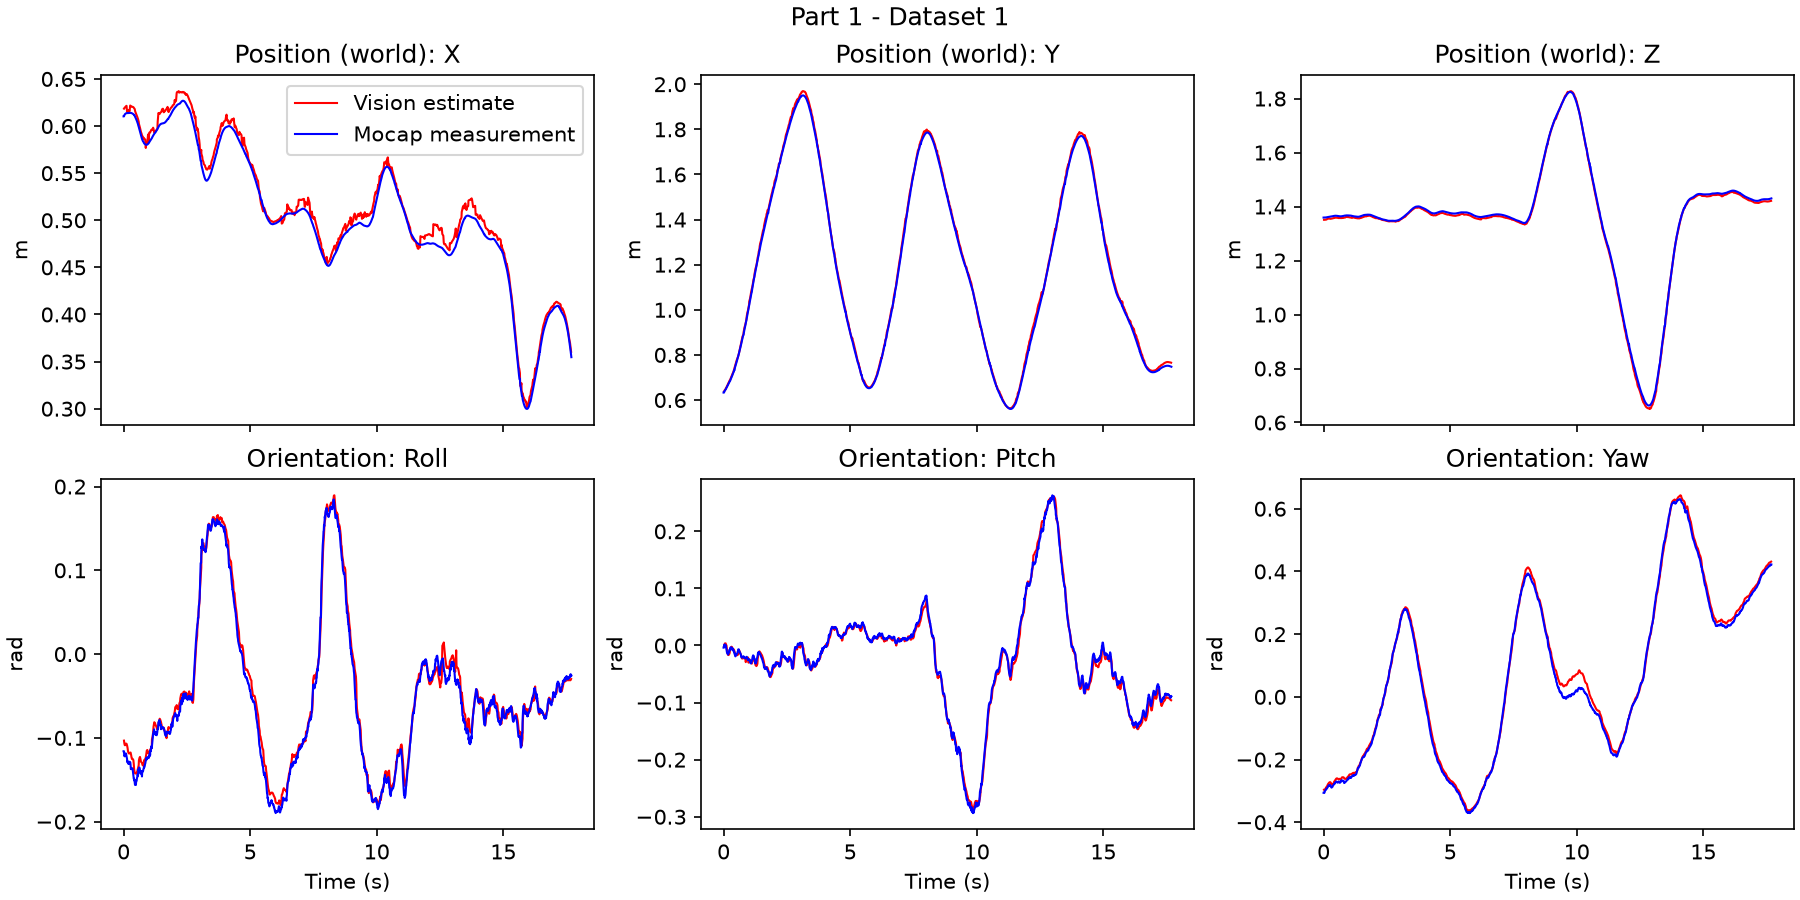
\includegraphics[width=0.79\textwidth]{figures/part1_dataset1.png}\\[0.2em]
  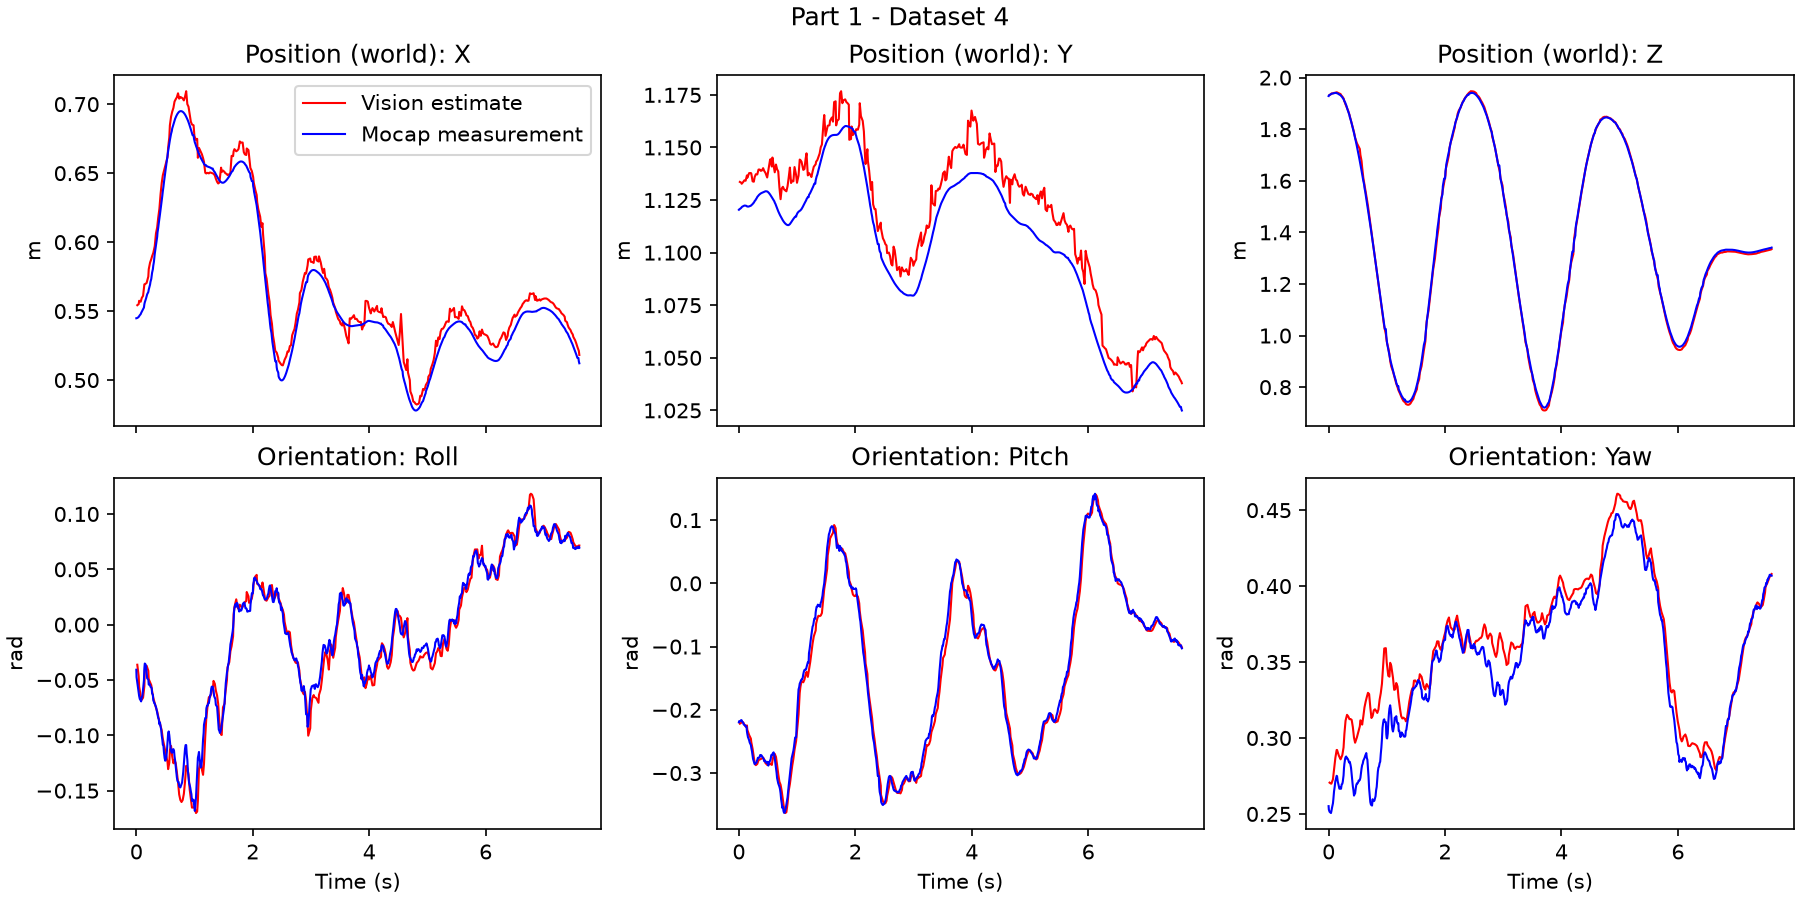
\includegraphics[width=0.79\textwidth]{figures/part1_dataset4.png}
  \caption{Part 1 pose estimates (red) against mocap (blue), dataset 1 above and dataset 4 below.}
  \label{fig:part1}
\end{figure}

%======================================================================
\section{Part 2 --- Velocity from Sparse Optical Flow}
%======================================================================

\subsection{Detection, tracking, and normalization}

For each consecutive pair we detect Shi--Tomasi corners in the \emph{previous} image with
\texttt{cv.goodFeaturesToTrack} and track them into the current image with the pyramidal
Lucas--Kanade tracker \texttt{cv.calcOpticalFlowPyrLK}, discarding tracks whose status flag is zero.
Corners are not restricted to the tags: the scribble between tags is high-texture and lies in the
same $Z=0$ plane, so it supplies well-conditioned features exactly where the tag grid is sparse.
Pixels are converted to calibrated coordinates by inverting $\mathbf{K}$,
\begin{equation}
x = \frac{u-c_u}{f_u},\quad y = \frac{v-c_v}{f_v},\qquad
[\dot x,\dot y]^{\mathsf T} = \frac{1}{\Delta t}\left[\frac{u'-u}{f_u},\ \frac{v'-v}{f_v}\right]^{\mathsf T},
\quad \Delta t = t_k-t_{k-1},
\end{equation}
which removes the intrinsics from the motion model so the fitted quantities are metric; $\dot
x,\dot y$ have units of $\mathrm{s}^{-1}$.

\subsection{Feature depth by ray--plane intersection}

The model needs each feature's camera-frame depth $Z$, which is neither the vehicle height nor the
distance along the ray but the point's camera-$z$ coordinate. Assuming every tracked feature lies on
the mat, we intersect the back-projected ray with $Z_W=0$ using the \emph{previous} frame's pose. A
point on the ray is $\vt{p}_C = Z[x,y,1]^{\mathsf T}$ and $\vt{p}_W = \Rwc\vt{p}_C+\vt{t}_{WC}$;
imposing $\vt{e}_3^{\mathsf T}\vt{p}_W=0$ gives
\begin{equation}
Z = \frac{-\,\vt{e}_3^{\mathsf T}\vt{t}_{WC}}{\vt{e}_3^{\mathsf T}\Rwc[x,y,1]^{\mathsf T}},
\qquad
\Rwc = \Rwb\Rcb^{\mathsf T},\qquad
\vt{t}_{WC} = \vt{p}_{WB}-\Rwc\vt{t}_{CB}.
\end{equation}
The numerator is the camera's height above the mat --- again obtained from the body position by
removing the lever arm, not by taking $\vt{p}_{WB,z}$ directly --- and the denominator is the
vertical component of the ray in world axes. Features with a vanishing denominator or $Z\le0$ (rays
that never strike the mat in front of the camera) are dropped along with their flow.

\subsection{Image motion model}

Let $\vt{V}$ and $\bm{\Omega}$ be the camera-origin linear velocity and the camera angular velocity,
both in the camera frame. For a world-static point the camera-frame coordinates evolve as
$\dot{\vt{p}}_C = -\vt{V}-\bm{\Omega}\times\vt{p}_C$. Differentiating $x=X/Z$, $y=Y/Z$ gives $\dot x
= \dot X/Z - x\dot Z/Z$ and $\dot y = \dot Y/Z - y\dot Z/Z$; substituting the components and
collecting terms yields the image-motion equations, linear in the six unknowns:
\begin{equation}
\begin{bmatrix}\dot{x}\\[1pt]\dot{y}\end{bmatrix}
=
\underbrace{\begin{bmatrix}
-\dfrac{1}{Z} & 0 & \dfrac{x}{Z} & xy & -(1+x^{2}) & y\\[7pt]
0 & -\dfrac{1}{Z} & \dfrac{y}{Z} & 1+y^{2} & -xy & -x
\end{bmatrix}}_{\mathbf{A}_i(x,y,Z)\,\in\,\mathbb{R}^{2\times6}}
\begin{bmatrix}V_x & V_y & V_z & \Omega_x & \Omega_y & \Omega_z\end{bmatrix}^{\mathsf T}.
\label{eq:flowmodel}
\end{equation}
The structure explains much of what follows. The translational block carries $1/Z$ --- translation
produces parallax, so near points move faster and depth is required --- whereas the rotational block
is depth-free. Rotation therefore carries no range information, and an interval that is mostly
rotational conditions the translation estimate poorly.

\subsection{Linear fit and transformation to body quantities}

Each retained track contributes two rows, so $n$ tracks give $\mathbf{A}\in\mathbb{R}^{2n\times6}$
and a stacked measurement $\vt{q}$. For $n\ge3$ we take
$\bm{\xi}^\star = \arg\min\norm{\mathbf{A}\bm{\xi}-\vt{q}}_2^2 = \mathbf{A}^{+}\vt{q}$ via the SVD
pseudo-inverse, truncating singular values below $10^{-10}$. The SVD form is preferred to the normal
equations because it degrades gracefully when a frame is near-degenerate, returning the minimum-norm
solution instead of amplifying noise through an ill-conditioned
$\mathbf{A}^{\mathsf T}\mathbf{A}$.

The fit is in camera quantities; the deliverables are body quantities. Camera and body are rigidly
attached, so they share an angular velocity and only its expression changes,
$\bm{\omega}_B = \Rcb^{\mathsf T}\bm{\Omega}$. For the linear term, differentiating
$\vt{p}_{WB} = \vt{t}_{WC}+\Rwc\vt{t}_{CB}$ with $\dot{\Rwc}=\Rwc\skewm{\bm{\Omega}}$ and
$\dot{\vt{t}}_{WC}=\Rwc\vt{V}$ gives
\begin{equation}
\boxed{\ \vt{v}_{WB} = \Rwc\left(\vt{V}+\bm{\Omega}\times\vt{t}_{CB}\right).\ }
\label{eq:leverarm}
\end{equation}
Rotation about the body origin sweeps the offset camera, so omitting
$\bm{\Omega}\times\vt{t}_{CB}$ is a systematic error proportional to angular rate: with
$\norm{\vt{t}_{CB}}=5\,$cm and body rates reaching $1.3\,$rad/s here it contributes up to
$6.5\,$cm/s, comparable to the total error budget.

\subsection{Three-point RANSAC}

Each correspondence gives two equations against six unknowns, so the minimal sample is $M=3$ points.
Each trial draws three distinct correspondences, rejects the sample if its $6\times6$ system is rank
deficient (three collinear or coincident features leave some degrees of freedom unconstrained), and
solves exactly. Every track is then scored by its two-component flow residual
$r_i = \norm{\mathbf{A}_i\bm{\xi}-[\dot x_i,\dot y_i]^{\mathsf T}}_2 < \tau$; the largest consensus
set is kept and the reported motion is a least-squares refit over \emph{all} of its inliers, since a
three-point fit is only a hypothesis generator and far too noisy to report directly. An interval
returns \texttt{None} if no trial reaches three inliers, and the plotter leaves a gap. The trial
count follows the standard coverage argument --- to draw at least one all-inlier sample with
probability $p$ when a fraction $\varepsilon$ of points are inliers,
\begin{equation}
N = \left\lceil \log(1-p)\,/\,\log\!\left(1-\varepsilon^{M}\right) \right\rceil .
\label{eq:iters}
\end{equation}

\subsection{Parameter choices}

\textbf{Inlier threshold.} The residual is a \emph{flow} residual, so its units are $\mathrm{s}^{-1}$
and its scale goes as $1/\Delta t$. A constant threshold in $\mathrm{s}^{-1}$ would therefore be a
much stricter test on a short interval than on a long one --- and as Section~\ref{sec:jitter} shows,
the intervals in these datasets vary by more than a factor of ten. We instead fix a tolerance on KLT
tracking error in \emph{pixels} and convert:
\begin{equation}
\tau = \frac{\epsilon_{\text{px}}}{f\,\Delta t},\qquad \epsilon_{\text{px}} = 0.3\ \text{px},
\qquad f = \tfrac12(f_u+f_v).
\end{equation}
At the median $20\,$ms interval this is $\tau\approx0.048\,\mathrm{s}^{-1}$. The value $0.3\,$px is
chosen to sit just above the sub-pixel accuracy of a $15\times15$ pyramidal KLT window: a tolerance
below the tracker's own noise floor rejects perfectly good measurements, which is the failure mode
visible in the first row of Table~\ref{tab:sweep}, where a $0.06\,$px budget leaves a consensus set
that is small, arbitrary, and a worse estimator than using every track.

\textbf{Trial count.} We take $\varepsilon=0.5$ and $p=0.99$ in \eqref{eq:iters}, giving $N=35$. The
observed inlier fraction at the chosen $\tau$ is far higher ($>0.95$), so this is deliberately
pessimistic. The reason extra trials still help is not the outlier rate but hypothesis quality: each
hypothesis comes from only three noisy points, so more draws means a better chance that some
consensus set is generated by a well-conditioned, low-noise triple. Table~\ref{tab:sweep} shows both
effects --- at a given $\tau$, raising $N$ helps, and at a given $N$, a realistic $\tau$ helps, and
neither alone is sufficient.

\textbf{Detector and tracker.} We use \texttt{maxCorners}~$=100$, \texttt{qualityLevel}~$=0.3$,
\texttt{minDistance}~$=7$, \texttt{blockSize}~$=7$, and a $15\times15$ KLT window with 2 pyramid
levels. The corner cap is the binding constraint: the detector returns a full 100 corners in
essentially every frame, so the quality level has little influence. We tested raising the cap, and
it does not help --- at \texttt{maxCorners}~$=300$, \texttt{qualityLevel}~$=0.01$ the mean track
count rises to about 297 but velocity RMSE is marginally \emph{worse} on both datasets, because the
additional corners are lower-contrast and track less reliably. 100 well-chosen features already
over-determine a six-parameter fit by a factor of thirty.

\begin{table}[htbp]
\centering\small
\caption{RANSAC parameter study, run end-to-end through the submitted estimator and scored against
mocap. Entries are linear-velocity RMSE $[v_x,v_y,v_z]$ in m/s. A pixel budget below the tracker's
noise floor is worse than no outlier rejection at all; the chosen setting is the last row.}
\label{tab:sweep}
\begin{tabular}{llcc}
\toprule
$\epsilon_{\text{px}}$ & $\varepsilon$ ($N$) & Dataset 1 & Dataset 4 \\
\midrule
\multicolumn{2}{l}{least squares, RANSAC off} & $[0.090,\ 0.300,\ 0.164]$ & $[0.106,\ 0.101,\ 0.503]$ \\
\midrule
0.06 & 0.8 \ (7)  & $[0.122,\ 0.331,\ 0.165]$ & $[0.337,\ 0.342,\ 0.501]$ \\
0.06 & 0.5 (35)   & $[0.070,\ 0.299,\ 0.165]$ & $[0.116,\ 0.104,\ 0.505]$ \\
0.30 & 0.8 \ (7)  & $[0.067,\ 0.300,\ 0.163]$ & $[0.137,\ 0.142,\ 0.500]$ \\
0.30 & 0.6 (19)   & $[0.067,\ 0.299,\ 0.163]$ & $[0.100,\ 0.085,\ 0.503]$ \\
\textbf{0.30} & \textbf{0.5 (35)} & $\bm{[0.067,\ 0.300,\ 0.163]}$ & $\bm{[0.089,\ 0.071,\ 0.503]}$ \\
\bottomrule
\end{tabular}
\end{table}

\subsection{Effect of timestamp jitter}
\label{sec:jitter}

Velocity is obtained by dividing a displacement by $\Delta t$, so any error in $\Delta t$ scales that
interval's entire velocity estimate multiplicatively. The image timestamps in these datasets are
badly jittered: the median interval is $20.0\,$ms, but the $5$--$95$ percentile range is
$8$--$31\,$ms and the extremes are $3\,$ms and $52\,$ms, a relative standard deviation of $33\%$.
The histogram in Figure~\ref{fig:jitter} is clustered near $10$, $20$ and $30\,$ms, which is the
signature of timestamps quantised to a coarser clock than the true frame interval rather than of a
genuinely variable frame rate.

The consequence is severe and asymmetric. If an interval's true spacing is $20\,$ms but it is
recorded as $8\,$ms, every flow vector is divided by a number $2.5\times$ too small and that sample's
velocity is inflated by $2.5\times$ --- which is exactly the spike pattern in the red traces of
Figures~\ref{fig:part2ds1} and \ref{fig:part2ds4}, where the estimate follows the mocap mean
faithfully but is punctuated by large outliers. The right panel of Figure~\ref{fig:jitter} confirms
the mechanism: the largest errors concentrate at short recorded $\Delta t$.

To quantify the contribution we re-ran the submitted estimator on frame pairs whose timestamps were
re-spaced to the median interval while holding each pair's midpoint fixed, so the mocap comparison is
untouched and only $\Delta t$ changes. RMS speed error falls by $5.5\times$ on dataset 1 and
$5.9\times$ on dataset 4:

\begin{center}\small
\begin{tabular}{llcc}
\toprule
 & & linear velocity RMSE (m/s) & angular velocity RMSE (rad/s) \\
\midrule
Dataset 1 & recorded $\Delta t$ & $[0.067,\ 0.300,\ 0.163]$ & $[0.166,\ 0.131,\ 0.183]$ \\
           & median $\Delta t$   & $[0.026,\ 0.055,\ 0.016]$ & $[0.061,\ 0.051,\ 0.038]$ \\
\midrule
Dataset 4 & recorded $\Delta t$ & $[0.087,\ 0.070,\ 0.500]$ & $[0.235,\ 0.301,\ 0.114]$ \\
           & median $\Delta t$   & $[0.047,\ 0.040,\ 0.060]$ & $[0.112,\ 0.086,\ 0.065]$ \\
\bottomrule
\end{tabular}
\end{center}

Timestamp jitter is therefore the \emph{dominant} error source in Part 2 --- larger than tracking
noise, the planar-scene assumption, and the pose error from Part 1 combined. We report the
recorded-$\Delta t$ results throughout, as the assignment specifies dividing by the elapsed image
time, but the comparison shows that the estimator itself is roughly five times more accurate than
the plots suggest, and that any downstream filter should either model the timing uncertainty or
recover a better frame clock.

\begin{figure}[htbp]
  \centering
  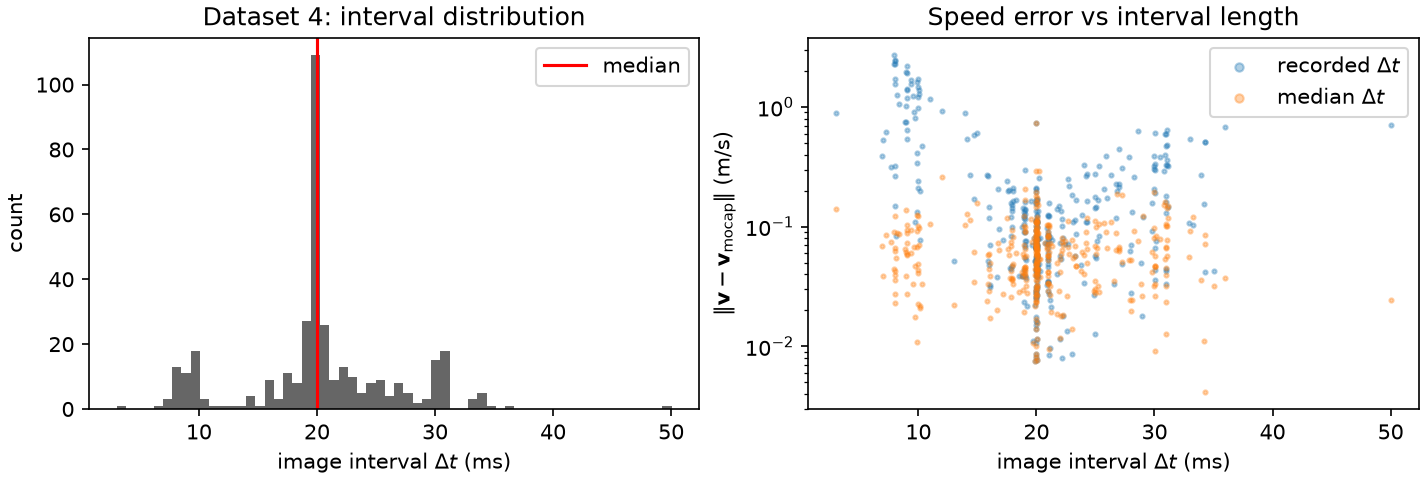
\includegraphics[width=0.66\textwidth]{figures/jitter_dataset4.png}
  \caption{Dataset 4 image-interval statistics. Left: the recorded intervals cluster near 10, 20 and
  30\,ms rather than forming a tight peak at the 20\,ms median. Right: per-interval speed error
  against interval length, with recorded and median $\Delta t$ overlaid; the large errors sit at
  short recorded intervals and largely vanish once $\Delta t$ is re-spaced.}
  \label{fig:jitter}
\end{figure}

\subsection{Part 2 results}

Table~\ref{tab:vel} gives velocity RMSE for both datasets with and without outlier rejection, and
Figures~\ref{fig:part2ds1}--\ref{fig:part2ds4} show the corresponding traces.

\begin{table}[htbp]
\centering\small
\caption{Part 2 RMS error against mocap, with and without RANSAC. All intervals produced an
estimate (863/863 and 372/372).}
\label{tab:vel}
\begin{tabular}{llcccccc}
\toprule
& & $v_x$ & $v_y$ & $v_z$ & $\omega_x$ & $\omega_y$ & $\omega_z$ \\
& & \multicolumn{3}{c}{(m/s)} & \multicolumn{3}{c}{(rad/s)} \\
\midrule
\multirow{2}{*}{Dataset 1} & least squares & 0.0897 & 0.2996 & 0.1645 & 0.1753 & 0.1469 & 0.1867 \\
 & RANSAC & \textbf{0.0668} & \textbf{0.2998} & \textbf{0.1630} & \textbf{0.1659} & \textbf{0.1308} & \textbf{0.1831} \\
\midrule
\multirow{2}{*}{Dataset 4} & least squares & 0.1056 & 0.1007 & 0.5028 & 0.2292 & 0.3189 & 0.1141 \\
 & RANSAC & \textbf{0.0864} & \textbf{0.0668} & \textbf{0.5011} & 0.2304 & \textbf{0.3010} & \textbf{0.1145} \\
\bottomrule
\end{tabular}
\end{table}

\textbf{Agreement with mocap.} The estimates track the mocap traces closely in shape and phase
across both runs; per-component correlation with the reference is $0.65$--$0.92$. The residual is
dominated by the interval-to-interval spikes analysed in Section~\ref{sec:jitter} rather than by any
bias, and the estimated signals are visibly noisier than, but centred on, the measured ones.

\textbf{Effect of outlier rejection.} RANSAC improves every linear-velocity component on both
datasets, by $26\%$ in $v_x$ on dataset 1 and by $18\%$ and $34\%$ in $v_x,v_y$ on dataset 4, and it
improves five of the six angular components; the one exception, $\omega_x$ on dataset 4, is a
$0.5\%$ regression and is a tie in practice. The improvement is real but moderate, and that is
consistent with the error budget: RANSAC removes tracks that violate the model --- features on the
quadrotor's own shadow, points that drifted onto a different structure, and any feature not actually
on the mat plane --- but it cannot help with an error that is common to \emph{every} track in an
interval. A mis-recorded $\Delta t$ scales all of that interval's flow vectors identically, so the
corrupted measurements remain perfectly self-consistent and are accepted as a unanimous consensus.
This is why the gains in Table~\ref{tab:vel} are tens of percent while fixing $\Delta t$ in
Section~\ref{sec:jitter} gains a factor of five or six.

\textbf{The $v_z$ channel.} $v_z$ is noticeably the worst component on dataset 4 ($0.50\,$m/s) and is
barely improved by RANSAC. This is structural rather than a defect. Dataset 4 is the more aggressive
flight, reaching $2.0\,$m/s against $0.94\,$m/s for dataset 1, and vertical motion is observed only
through the looming term $\tfrac{x}{Z}V_z$, $\tfrac{y}{Z}V_z$ in \eqref{eq:flowmodel}. That term
vanishes at the image centre and grows only linearly towards the edges, so with a narrow
$376\times240$ field of view the whole estimate rests on a small differential signal --- and it is
precisely the component most amplified by a $\Delta t$ error. Consistently, $v_z$ is also the
component that improves most dramatically under the fixed-clock experiment, from $0.500$ to
$0.060\,$m/s.

\begin{figure}[htbp]
  \centering
  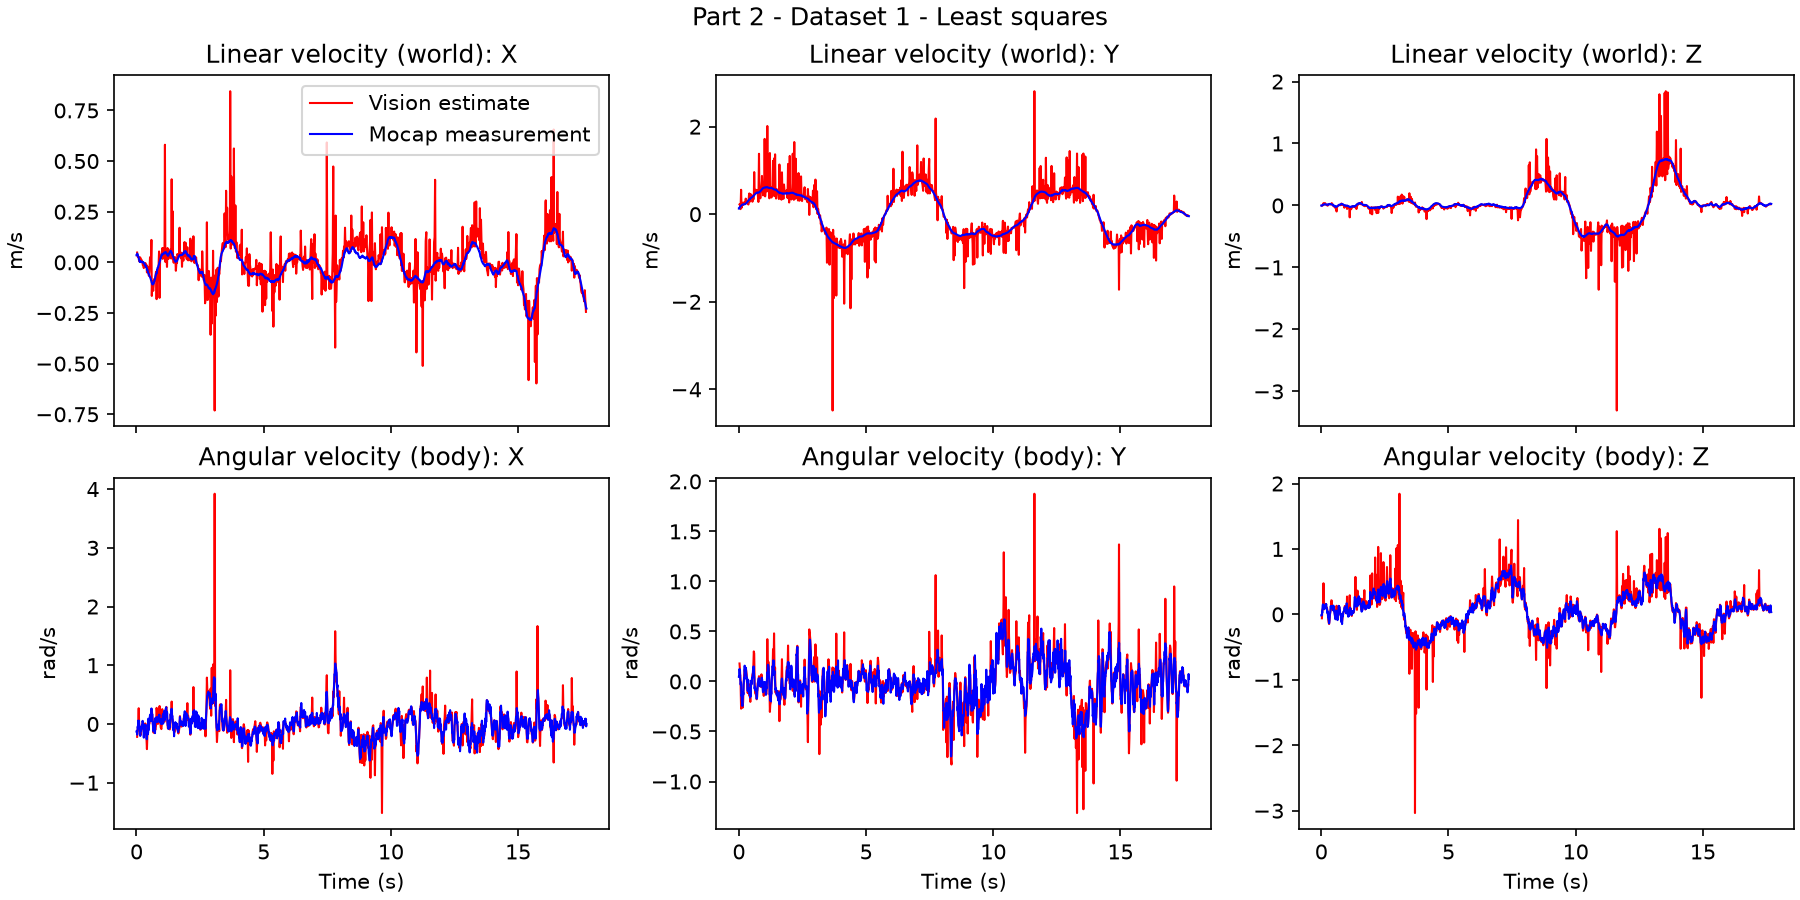
\includegraphics[width=0.79\textwidth]{figures/part2_lsq_dataset1.png}\\[0.2em]
  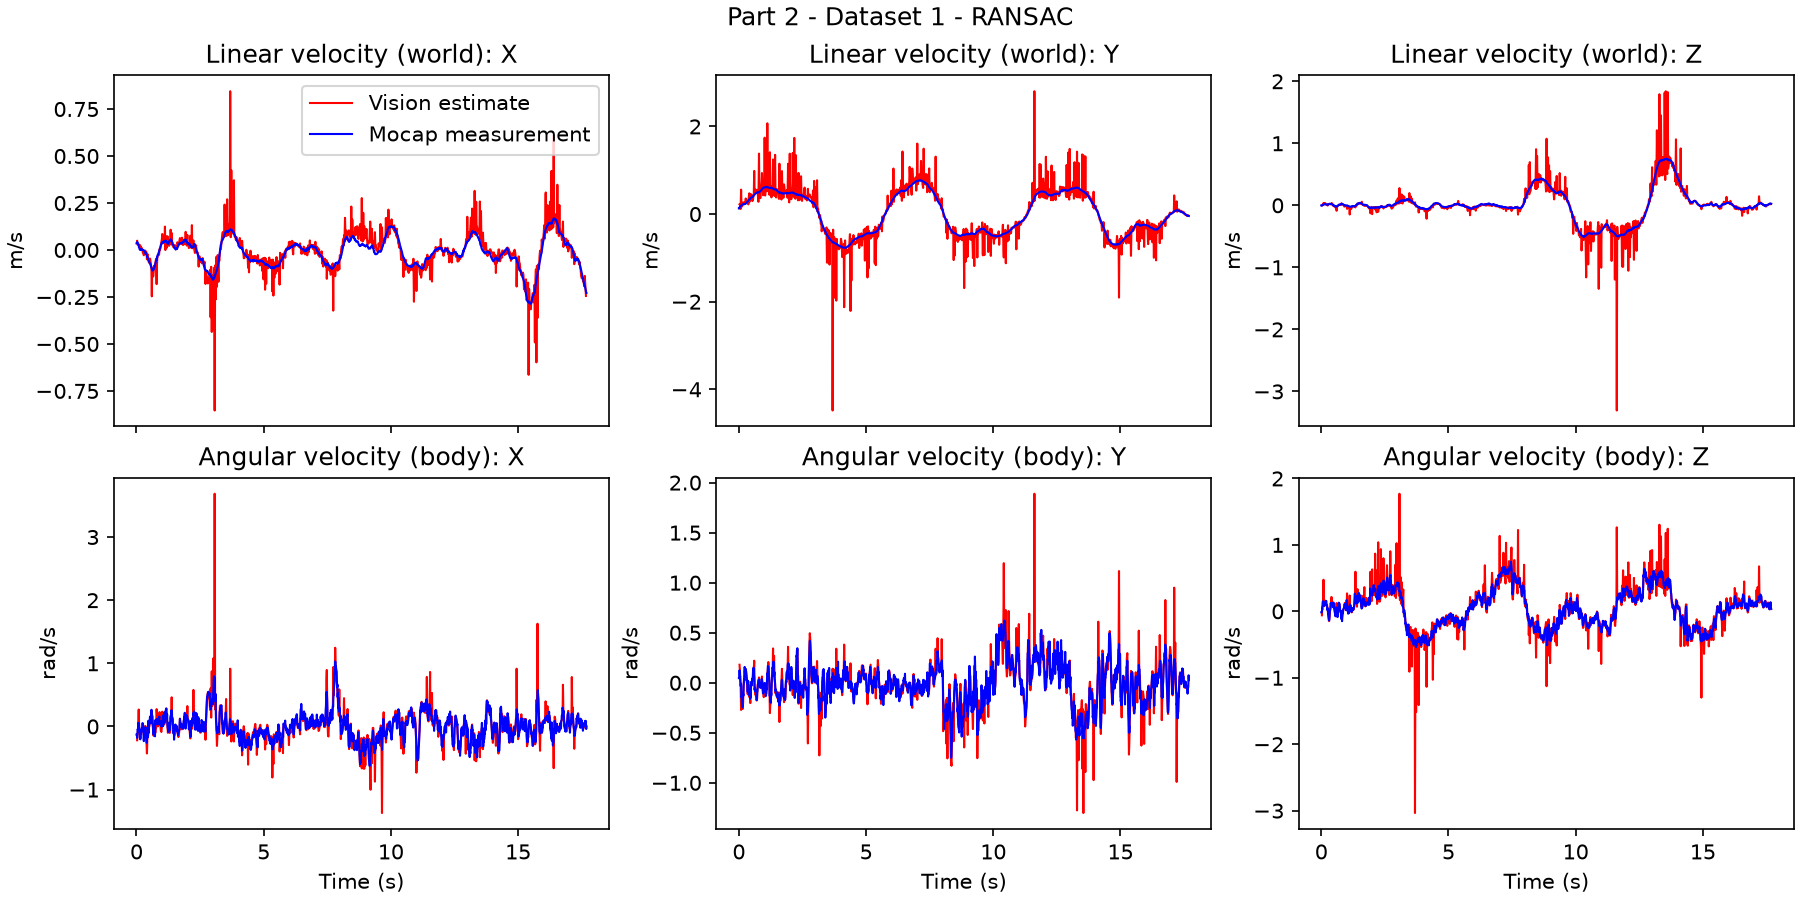
\includegraphics[width=0.79\textwidth]{figures/part2_ransac_dataset1.png}
  \caption{Dataset 1 velocity: least squares (above) and RANSAC (below).}
  \label{fig:part2ds1}
\end{figure}

\begin{figure}[htbp]
  \centering
  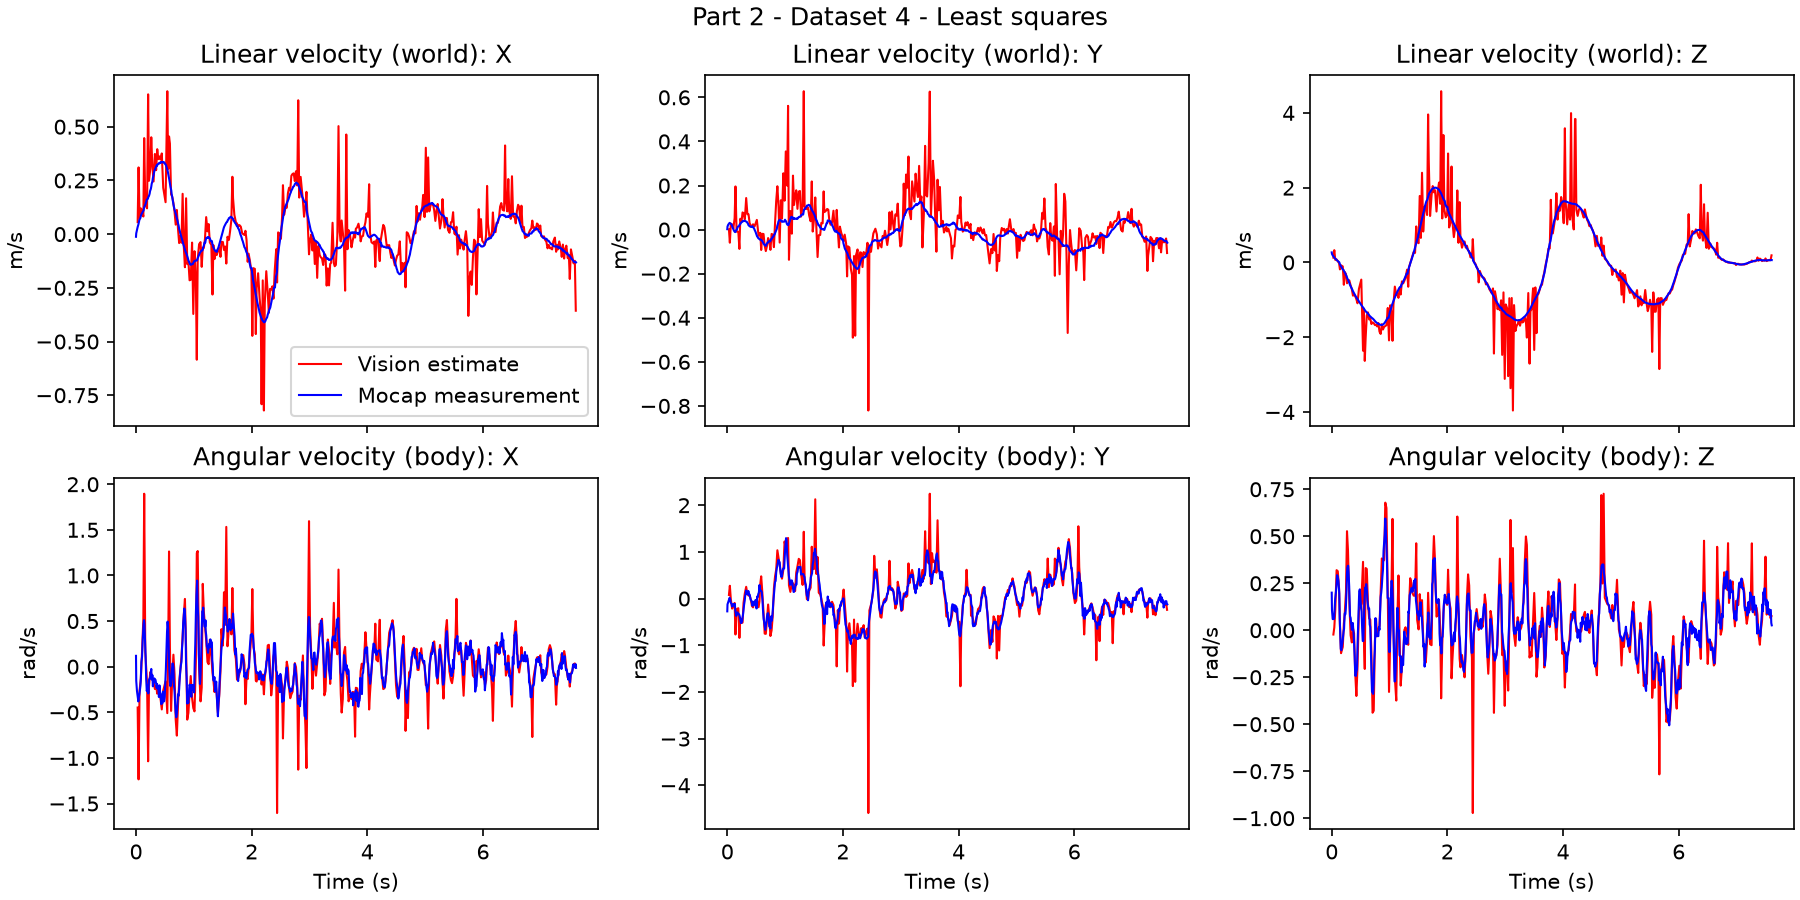
\includegraphics[width=0.79\textwidth]{figures/part2_lsq_dataset4.png}\\[0.2em]
  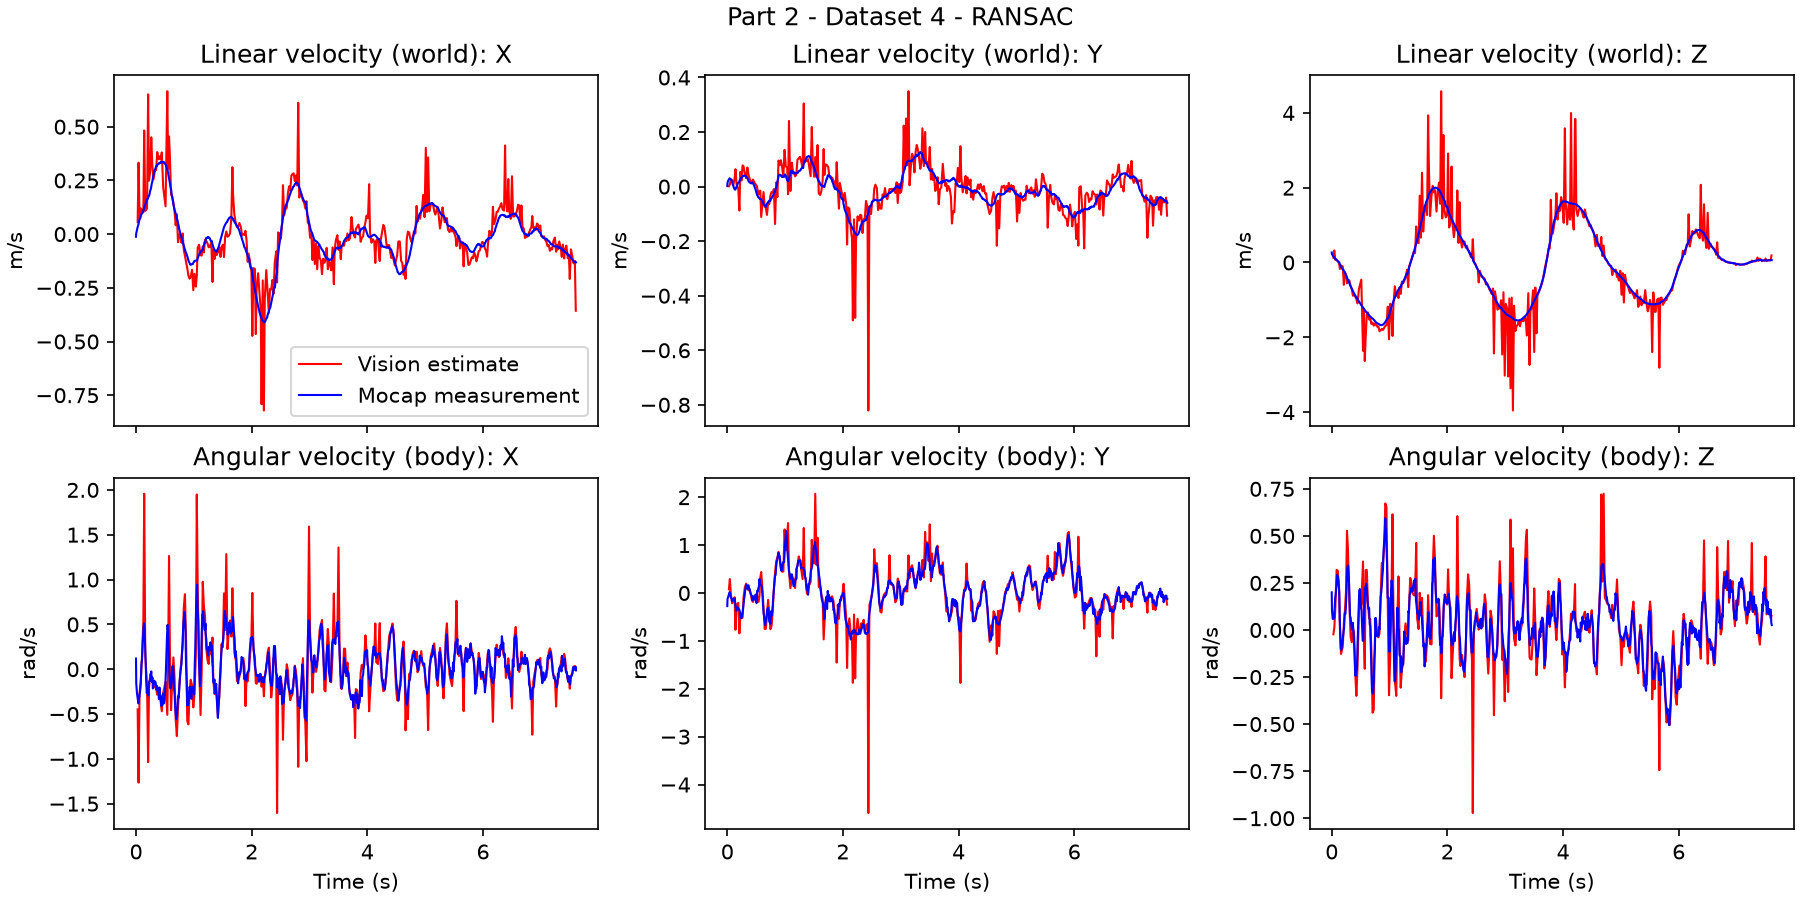
\includegraphics[width=0.79\textwidth]{figures/part2_ransac_dataset4.png}
  \caption{Dataset 4 velocity: least squares (above) and RANSAC (below).}
  \label{fig:part2ds4}
\end{figure}

%======================================================================
\section{Implementation Notes and Runtime}
%======================================================================

All estimation is implemented directly in \texttt{pose.py} and \texttt{flow.py}: the homography DLT
and its decomposition, the velocity fit, and RANSAC are written out rather than taken from a
library; only corner detection and KLT tracking use OpenCV, as permitted. Two details are worth
recording. The RANSAC residual is evaluated by forming the full $2n\times6$ design matrix once per
interval and scoring every hypothesis with a single matrix product, rather than rebuilding a
$2\times6$ block per point per trial; this is what makes $N=35$ trials affordable. The minimal-sample
draw is also bounded: if 20 consecutive draws are rank deficient the trial is abandoned, so a
degenerate interval cannot stall the run.

Measured wall-clock time for \texttt{run\_estimation()}, excluding loading and plotting, is
$0.26\,$s and $0.14\,$s for Part 1 and $3.58\,$s and $1.52\,$s for Part 2 with RANSAC on datasets 1
and 4 respectively --- comfortably inside the one-minute budget.

%======================================================================
\section{Conclusion}
%======================================================================

Pose recovery from a single planar homography per frame reproduces the mocap trajectory to about
$1\,$cm and $1^\circ$ over both datasets, with no filtering and no temporal smoothing, confirming
that the tag geometry, the scale and cheirality resolution, and the camera-to-body transformation
are all correctly handled. Velocity from KLT flow recovers the correct shape and magnitude of both
the linear and angular motion, and three-point RANSAC gives a consistent if moderate improvement
over an unweighted least-squares fit once its threshold is expressed as a pixel budget rather than a
fixed rate. The clearest lesson from the exercise is that the limiting factor is not the geometry
but the clock: the recorded image timestamps, not the tracker or the estimator, account for roughly
a factor of five in the final velocity error.

\end{document}
